\documentclass[11pt,a4paper]{article}
\usepackage[T1]{fontenc}
\usepackage{lmodern}
\usepackage[utf8]{inputenc}
\usepackage[margin=2.5cm]{geometry}
\usepackage{amsmath}
\usepackage{graphicx}
\usepackage{booktabs}
\usepackage{xcolor}
\usepackage{listings}
\usepackage{caption}
\usepackage{float}
\usepackage[round]{natbib}
\usepackage[hidelinks]{hyperref}
\usepackage{xurl}
\sloppy

\captionsetup{font=small,labelfont=bf}
\graphicspath{{../}}

\lstset{
  basicstyle=\ttfamily\footnotesize,
  backgroundcolor=\color{gray!8},
  frame=single, rulecolor=\color{gray!40},
  breaklines=true, postbreak=\mbox{\textcolor{gray}{$\hookrightarrow$}\space},
  columns=fullflexible, keepspaces=true, showstringspaces=false,
  upquote=true, literate={×}{{$\times$}}1 {–}{{--}}1 {−}{{-}}1 {χ}{{$\chi$}}1 {Γ}{{$\Gamma$}}1 {α}{{$\alpha$}}1 {σ}{{$\sigma$}}1 {ν}{{$\nu$}}1 {μ}{{$\mu$}}1 {²}{{$^2$}}1
}

\newcommand{\nh}{N_{\rm H}}
\newcommand{\cgs}{erg\,cm$^{-2}$\,s$^{-1}$}

\title{XMM-Newton Observation of the AGN 3C\,111\\[4pt]
\large Part C: X-ray Spectral Analysis with SAS and XSPEC}
\author{Panchatapa Pal}
\date{November 3, 2026}

\begin{document}
\maketitle

\begin{abstract}
I present the spectral analysis of the XMM-Newton EPIC-pn observation of the broad-line radio galaxy 3C\,111 (ObsID 0552180101). Starting from the cleaned event list, good time intervals and extraction regions of Part~A, source and background spectra were extracted with SAS~22.1.0, and redistribution (RMF) and ancillary (ARF) response files were generated. The source has a net count rate of $8.19\pm0.01$\,counts\,s$^{-1}$ in a livetime of 42.2\,ks, with the background contributing less than 1 per cent and no significant pile-up. The 0.3--10\,keV spectrum was fitted in XSPEC. An absorbed power law gives $\nh=(1.054\pm0.009)\times10^{22}$\,cm$^{-2}$ and $\Gamma=1.627\pm0.008$, but leaves a clear excess near 6.1\,keV (observed frame). Adding a Gaussian emission line improves the fit by $\Delta\chi^2=45.6$ for three additional parameters; the line has a rest-frame energy of $6.38\pm0.05$\,keV, consistent with neutral Fe\,K$\alpha$, and an equivalent width of $41\pm12$\,eV. For this best-fitting model the observed and unabsorbed 2--10\,keV fluxes are $4.59\times10^{-11}$ and $4.86\times10^{-11}$\,\cgs, and the rest-frame 2--10\,keV luminosity is $(2.70\pm0.01)\times10^{44}$\,erg\,s$^{-1}$. The residual excess in $\chi^2$ is confined below 3\,keV and is attributed to calibration effects at the high count rate; the 3--10\,keV band alone is fitted with $\chi^2/\mathrm{dof}=108.6/106$.
\end{abstract}

\tableofcontents

\section{Introduction}

The X-ray spectrum of an active galactic nucleus (AGN) is, to first order, a power law $N(E)\propto E^{-\Gamma}$, produced when ultraviolet photons from the accretion disc are Compton up-scattered by a hot corona of electrons above the disc. The photon index $\Gamma$ encodes the temperature and optical depth of the corona. Along its way to the observer the power law is modified by photoelectric absorption in cold gas, both in the host galaxy and in the Milky Way, which removes soft X-rays and is characterised by the equivalent hydrogen column density $\nh$. Part of the primary continuum is also reprocessed by surrounding matter, producing a fluorescent Fe\,K$\alpha$ emission line at 6.4\,keV (rest frame) and a reflection continuum. Fitting these components to the observed spectrum yields the intrinsic properties of the source.

3C\,111 is a nearby ($z=0.049$) broad-line radio galaxy with a powerful one-sided relativistic jet, located at low Galactic latitude behind a large column of Galactic gas. Its X-ray spectrum is therefore expected to be strongly absorbed at low energies.

\paragraph{Objective of Part C.} Extract the source and background spectra from the cleaned EPIC-pn data, generate the response files (RMF and ARF), plot the spectrum, fit it with an absorbed X-ray spectral model in XSPEC, and determine the best-fit spectral parameters: hydrogen column density $\nh$, photon index $\Gamma$, normalisation, observed and unabsorbed fluxes, X-ray luminosity, flux density, and the fit statistic.

\section{Input Data and Software}

The analysis starts from the products of Part~A (Table~\ref{tab:input}). Table~\ref{tab:software} lists the software used.

\begin{table}[H]
\centering
\caption{Input products from Part A.}
\label{tab:input}
\begin{tabular}{ll}
\toprule
Clean event list & \texttt{pn\_clean.fits} (461\,931 events, CCD 4) \\
Good time intervals & extension \texttt{GTI00003} of \texttt{pn\_clean.fits}, 20 intervals, 60.3\,ks \\
Observing mode & EPIC-pn PrimeSmallWindow, Thin1 filter \\
Source region & circle, centre $(X,Y)=(27308.7,\,27578.4)$, $r=30''$ (600 sky units) \\
Background region & circle, centre $(X,Y)=(25689,\,24313)$, $r=40''$ (800 sky units) \\
Calibration index & \texttt{ccf.cif} (129 CCF entries) \\
\bottomrule
\end{tabular}
\end{table}

\begin{table}[H]
\centering
\caption{Software used.}
\label{tab:software}
\begin{tabular}{ll}
\toprule
SAS & 22.1.0 (Ubuntu 24.04 build) \\
XSPEC & 13 (HEASoft) \\
Python & 3.12 with \texttt{astropy}, \texttt{numpy}, \texttt{matplotlib} \\
Plotting & \texttt{matplotlib}; \texttt{pymupdf} to read the \texttt{epatplot} output \\
\bottomrule
\end{tabular}
\end{table}

\paragraph{Calibration files.} The SAS response tasks read many Current Calibration Files (CCFs) that were not needed in Part~A. The missing EPIC-pn, mirror (\texttt{XRT3\_XAREAEF}, \texttt{XRT3\_XENCIREN}) and general XMM CCFs listed in \texttt{ccf.cif} were downloaded from the HEASARC mirror before the responses could be generated. Because the ODF summary file copied into the working directory was truncated and could not be re-ingested by \texttt{cifbuild}, the calibration index of Part~A was reused; it was built for the observation date and is therefore valid.

\section{Spectral Extraction}

\subsection{Source and background spectra}

Spectra were extracted with \texttt{evselect} from the clean event list, using the regions and good time intervals of Part~A. Only events from CCD~4 with \texttt{FLAG==0} and \texttt{PATTERN<=4} (singles and doubles) were accepted. The spectra cover the standard pn channel range 0--20479 with a bin size of 5:

\begin{lstlisting}[language=bash]
evselect table=pn_clean.fits:EVENTS withspectrumset=yes spectrumset=pn_src_spec.pi \
  energycolumn=PI spectralbinsize=5 withspecranges=yes specchannelmin=0 specchannelmax=20479 \
  expression="(CCDNR==4)&&(FLAG==0)&&(PATTERN<=4)&&((X,Y) IN circle(27308.7,27578.4,600))&&gti(pn_clean.fits:GTI00003,TIME)"
\end{lstlisting}

The background spectrum was extracted with the same command, using \texttt{circle(25689,24313,800)} and \texttt{spectrumset=pn\_bkg\_spec.pi}. The source region contains 348\,014 events and the background region 3\,579 events.

\subsection{Area scaling}

The task \texttt{backscale} computes the effective extraction area of each region, taking bad pixels and chip gaps into account, and writes it to the \texttt{BACKSCAL} keyword:

\begin{lstlisting}[language=bash]
backscale spectrumset=pn_src_spec.pi badpixlocation=pn_clean.fits
backscale spectrumset=pn_bkg_spec.pi badpixlocation=pn_clean.fits
\end{lstlisting}

The values are $1\,132\,600$ (source) and $2\,010\,700$ (background); their ratio, 0.563, equals $(30/40)^2$ as expected for two unobstructed circles. Scaled to the source area, the background contributes about 2\,000 counts, or 0.6 per cent of the source spectrum. Background subtraction therefore has a negligible effect on the results.

\subsection{Response files}

The redistribution matrix file (RMF) describes how a photon of a given energy is distributed over detector channels; the ancillary response file (ARF) gives the effective area as a function of energy, including mirror area, filter transmission, quantum efficiency and the fraction of the point-spread function (PSF) enclosed by the source region:

\begin{lstlisting}[language=bash]
rmfgen spectrumset=pn_src_spec.pi rmfset=pn_src.rmf withenergybins=yes \
  energymin=0.1 energymax=12 nenergybins=2400
arfgen spectrumset=pn_src_spec.pi arfset=pn_src.arf withrmfset=yes rmfset=pn_src.rmf \
  badpixlocation=pn_clean.fits detmaptype=psf
\end{lstlisting}

The RMF has 2400 energy bins between 0.1 and 12\,keV. The ARF was computed for a point source at the off-axis angle of 3C\,111 ($\theta=67.9''$), using the elliptical-beta PSF model; the fraction of the source region lost to bad pixels and chip gaps is negligible. Because the source region ($r=30''$) does not enclose the whole PSF, the ARF corrects the flux for the missing PSF wings.

\subsection{Grouping}

To make $\chi^2$ statistics valid, the spectrum was grouped with \texttt{specgroup} to at least 25 counts per bin, without oversampling the instrumental energy resolution by more than a factor of 3:

\begin{lstlisting}[language=bash]
specgroup spectrumset=pn_src_spec.pi mincounts=25 oversample=3 rmfset=pn_src.rmf \
  arfset=pn_src.arf backgndset=pn_bkg_spec.pi groupedset=pn_src_grp.pi
\end{lstlisting}

The grouped spectrum \texttt{pn\_src\_grp.pi} has 218 groups, of which 177 lie in the fitted 0.3--10\,keV band. The background, RMF and ARF file names are stored in its header keywords \texttt{BACKFILE}, \texttt{RESPFILE} and \texttt{ANCRFILE}, so XSPEC loads them automatically.

\subsection{Pile-up check}

The source count rate is about 8\,counts\,s$^{-1}$, so I checked for pile-up before fitting. When two photons land in the same frame close to each other, they are read out as one event with a larger pattern. Pile-up therefore lowers the fraction of single events and raises the fraction of doubles compared with what is expected.

I ran \texttt{epatplot} on the source events (Fig.~\ref{fig:epat}a). In 0.5--2\,keV it gives observed-to-model ratios of $s=1.026\pm0.004$ for singles and $d=1.014\pm0.006$ for doubles. Both are above 1, which at first looks odd since the fractions have to add up to one. The reason is that the clean event list from Part~A only has \texttt{PATTERN<=4}. There are no triples or quadruples left in the data (their observed fractions in Fig.~\ref{fig:epat}a are zero), but the \texttt{epatplot} model still expects about 2 per cent of them. So the singles and doubles come out slightly high in both cases.

To compare like with like, I read the observed and expected fractions from the \texttt{epatplot} output and renormalised the expected curves to singles plus doubles only (Fig.~\ref{fig:epat}b). With this, the observed fractions follow the expected ones over the full energy range. In 0.5--2\,keV the ratios are 1.015 for singles and 0.96 for doubles. This is a small deficit of doubles, which is the opposite of what pile-up would do. Part~A ran \texttt{epatplot} on the unscreened events with all patterns and got $s=1.003\pm0.004$ and $d=0.991\pm0.005$. I conclude that the spectrum is not piled up, and I used the full $30''$ source circle. The small shift from doubles to singles is discussed again in Section~\ref{sec:quality}.

\begin{figure}[!htbp]
\centering
\begin{minipage}[b]{0.49\textwidth}
\centering
\includegraphics[page=2,width=\linewidth]{figures/fig06_epatplot_pileup.pdf}\\
{\small (a)}
\end{minipage}\hfill
\begin{minipage}[b]{0.49\textwidth}
\centering
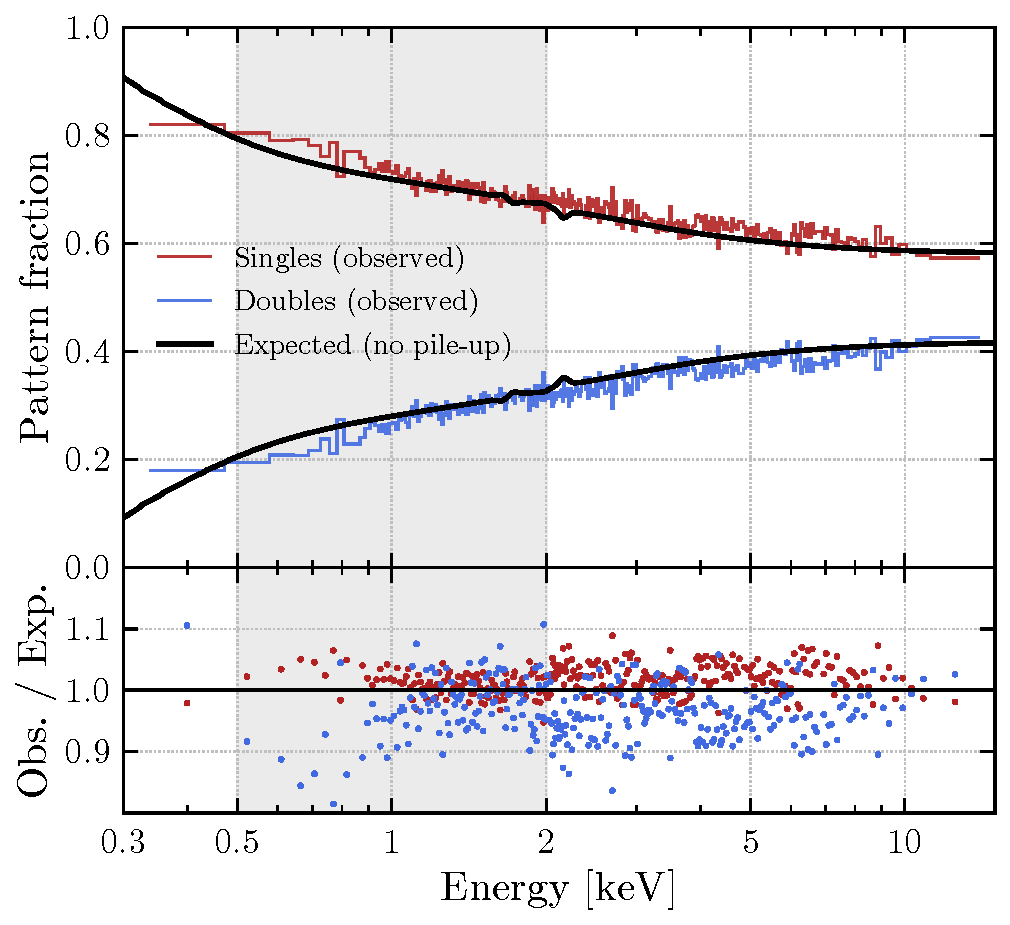
\includegraphics[width=\linewidth]{figures/fig06_pattern_fractions.pdf}\\
{\small (b)}
\end{minipage}
\caption{Pile-up check for the source region. (a) Output of \texttt{epatplot}. The histograms are the observed pattern fractions and the smooth curves are the fractions expected without pile-up, for singles (s), doubles (d), triples (t), quadruples (q) and singles plus doubles (s+d). (b) Observed single and double fractions compared with the expected fractions renormalised to singles plus doubles, since the clean event list has only \texttt{PATTERN<=4}. The lower panel shows the ratio of observed to expected fractions. The grey band is 0.5--2\,keV, the range used by \texttt{epatplot} for the pile-up test.}
\label{fig:epat}
\end{figure}

\subsection{Extracted spectrum}

The net (background-subtracted) count rate is $8.192\pm0.014$\,counts\,s$^{-1}$ in a livetime of 42\,234\,s, corresponding to about $3.5\times10^5$ net source counts. The livetime is shorter than the 60.3\,ks good-time interval because of the Small Window dead time (livetime fraction $\approx$71 per cent). Fig.~\ref{fig:spec} shows the spectrum. The strong low-energy cut-off below $\sim$1\,keV is produced by photoelectric absorption combined with the falling effective area; the sharp drops near 1.8 and 2.2\,keV are instrumental edges (Si K and the Au M edges of the mirror coating) that are folded into the response. A weak excess is visible near 6.1\,keV.

\begin{figure}[!htbp]
\centering
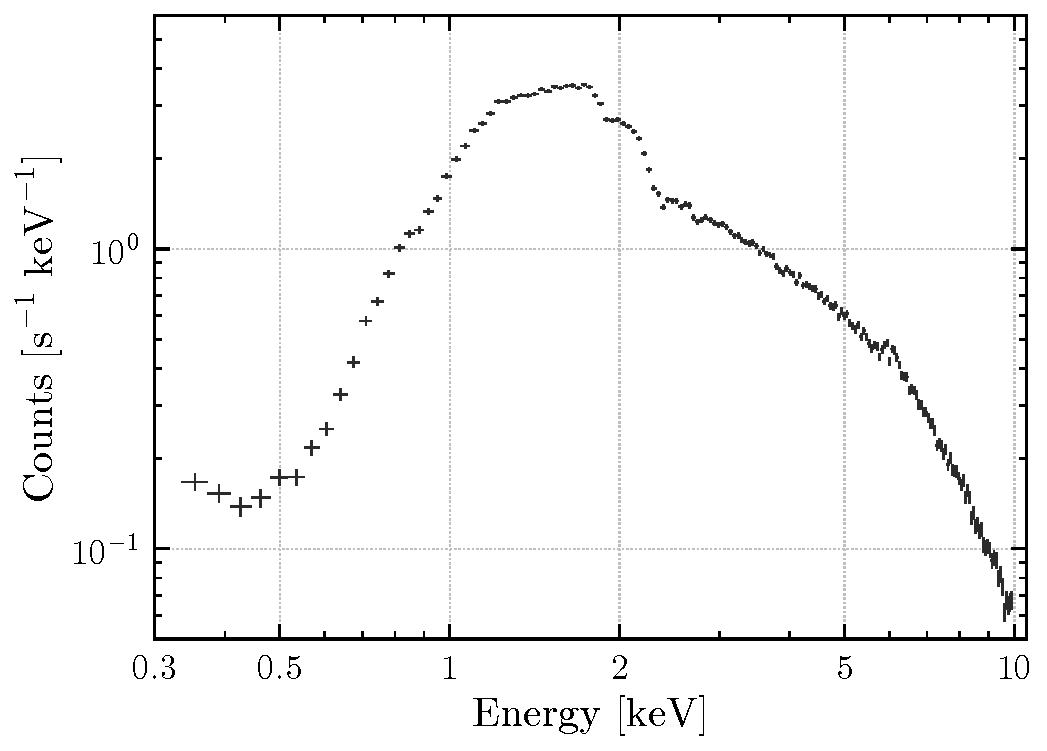
\includegraphics[width=0.72\textwidth]{figures/fig01_spectrum.pdf}
\caption{Background-subtracted XMM-Newton EPIC-pn spectrum of 3C\,111 (ObsID 0552180101), grouped to a minimum of 25 counts per bin.}
\label{fig:spec}
\end{figure}

\section{Spectral Fitting}

\subsection{Method}

Data products were made with SAS \citep{gabriel04}. All fits were performed in XSPEC \citep{arnaud96} over 0.3--10\,keV with $\chi^2$ statistics. Absorption was described with the Tübingen--Boulder model \texttt{tbabs} with the abundances of \cite{wilms00} and the cross-sections of \cite{verner96}. A single absorber was used for the Galactic and any intrinsic absorption, since the two cannot be separated at the resolution of the pn camera. The continuum was modelled with \texttt{zpowerlw}, a power law at the redshift of 3C\,111 ($z=0.049$, frozen). Errors are 90 per cent confidence intervals for one parameter of interest ($\Delta\chi^2=2.706$). Because the reduced $\chi^2$ exceeds 2, XSPEC's default limit for error calculation was raised with \texttt{error maximum 10.0}. A flat $\Lambda$CDM cosmology with $H_0=70$\,km\,s$^{-1}$\,Mpc$^{-1}$, $\Omega_\Lambda=0.73$ was adopted (\texttt{cosmo 70 0 0.73}), giving a luminosity distance $D_L=217.9$\,Mpc.

The complete XSPEC script is given in Appendix~\ref{app:scripts}.

\subsection{Absorbed power law}

The first model is the absorbed power law \texttt{tbabs$\times$zpowerlw}. The best fit gives $\nh=(1.054\pm0.009)\times10^{22}$\,cm$^{-2}$ and $\Gamma=1.627\pm0.008$, with $\chi^2/\mathrm{dof}=433.9/174$ (Fig.~\ref{fig:fitpl}). The model reproduces the overall shape of the spectrum, but the residuals show a significant excess around 6\,keV. The data-to-model ratio (Fig.~\ref{fig:ratio}) makes the feature clearer: an excess of about 10--12 per cent at 5.9--6.2\,keV, at the observed-frame energy of neutral Fe\,K$\alpha$, $6.4/(1+z)=6.10$\,keV.

\begin{figure}[!htbp]
\centering
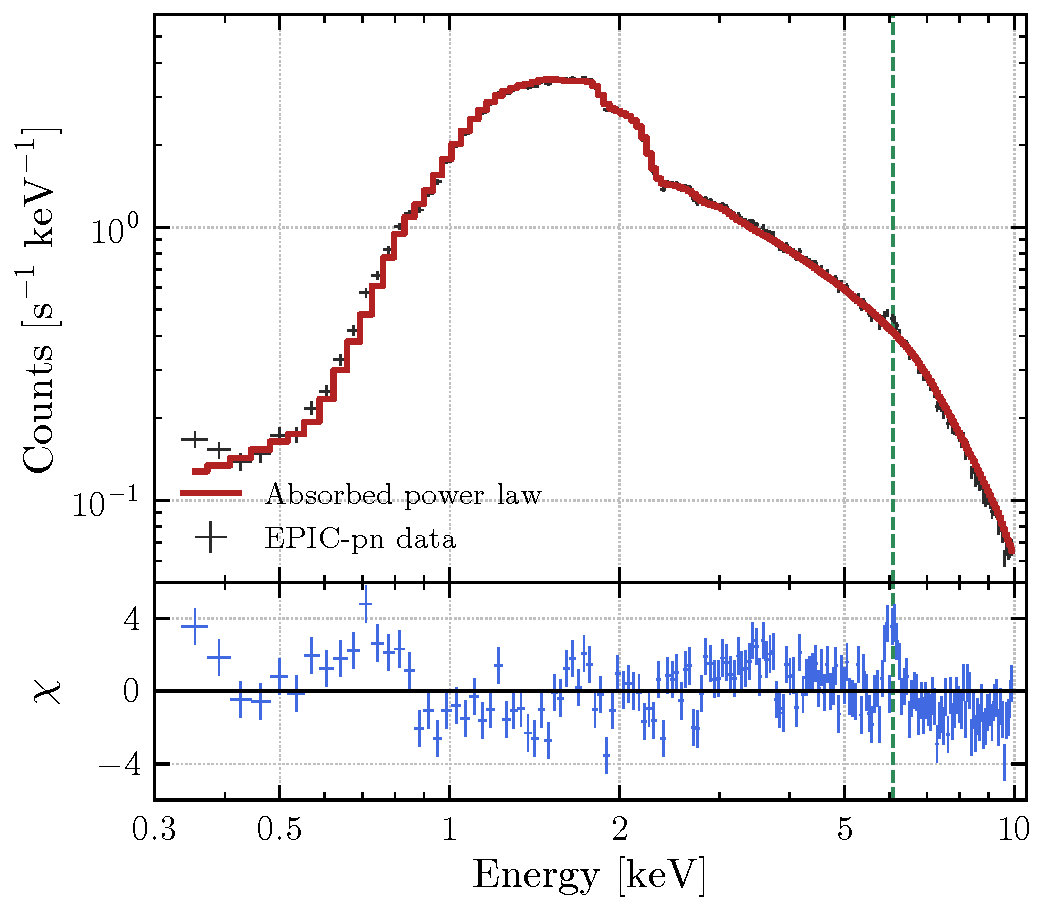
\includegraphics[width=0.72\textwidth]{figures/fig02_fit_absorbed_powerlaw.pdf}
\caption{EPIC-pn spectrum fitted with an absorbed power law (\texttt{tbabs$\times$zpowerlw}, $z=0.049$) in the 0.3--10\,keV band. The dashed line marks the observed-frame energy of neutral Fe\,K$\alpha$ (6.10\,keV). Lower panel: residuals in units of $\sigma$.}
\label{fig:fitpl}
\end{figure}

\begin{figure}[!htbp]
\centering
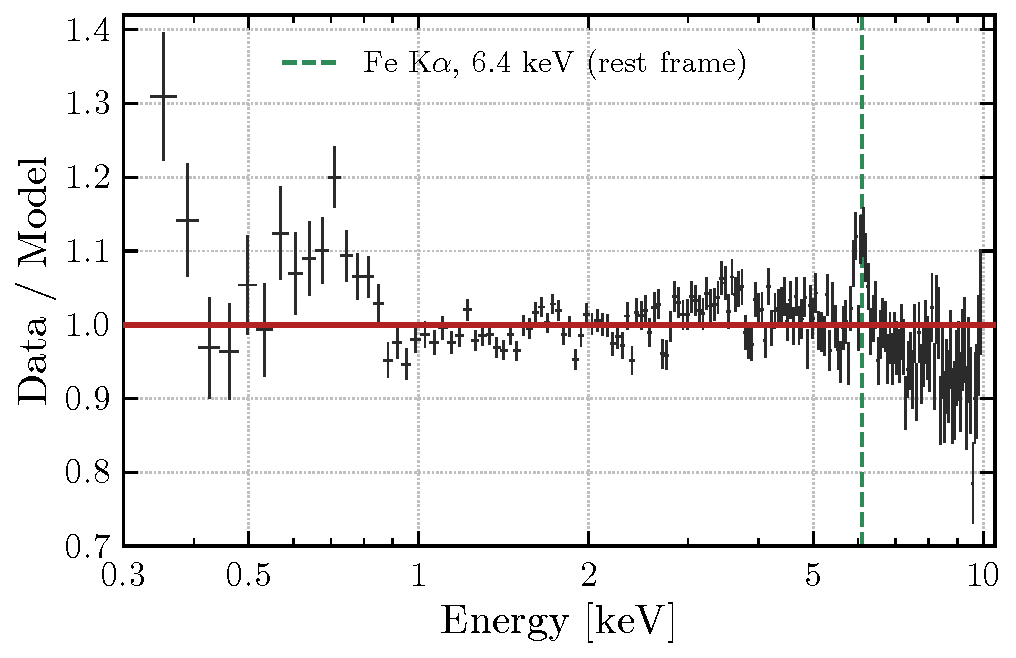
\includegraphics[width=0.75\textwidth]{figures/fig03_ratio_absorbed_powerlaw.pdf}
\caption{Data-to-model ratio for the absorbed power-law fit. The dashed line marks the expected energy of the neutral Fe\,K$\alpha$ line (6.4\,keV in the rest frame, 6.10\,keV observed).}
\label{fig:ratio}
\end{figure}

\subsection{Absorbed power law with an Fe\,K\texorpdfstring{$\alpha$}{alpha} line}

A redshifted Gaussian emission line (\texttt{zgauss}) was added, giving the model \texttt{tbabs$\times$(zpowerlw+zgauss)}. The line energy was allowed to vary between 5.8 and 7.2\,keV and the width up to 0.5\,keV. The fit improves to $\chi^2/\mathrm{dof}=388.3/171$, i.e.\ $\Delta\chi^2=45.6$ for three additional free parameters; an F-test gives a probability of $3\times10^{-4}$ that the improvement is due to chance.\footnote{The F-test is only approximate for testing the presence of an emission line \citep{protassov02}; given the size of $\Delta\chi^2$, the detection is nevertheless robust.} The line has a rest-frame energy of $6.378^{+0.050}_{-0.051}$\,keV, consistent with K$\alpha$ fluorescence from neutral or weakly ionised iron, and an equivalent width of $41\pm12$\,eV. It is marginally resolved, with $\sigma=0.124\pm0.055$\,keV, corresponding to a full width at half maximum of $\approx$13\,700\,km\,s$^{-1}$ (90 per cent range 7\,700--19\,800\,km\,s$^{-1}$). The continuum parameters are almost unchanged: $\nh=(1.058\pm0.009)\times10^{22}$\,cm$^{-2}$ and $\Gamma=1.635\pm0.008$. The excess at 6\,keV disappears from the residuals (Fig.~\ref{fig:fitfe}). This model is adopted as the best fit. Its unfolded spectrum is shown in Fig.~\ref{fig:unf}.

\begin{figure}[!htbp]
\centering
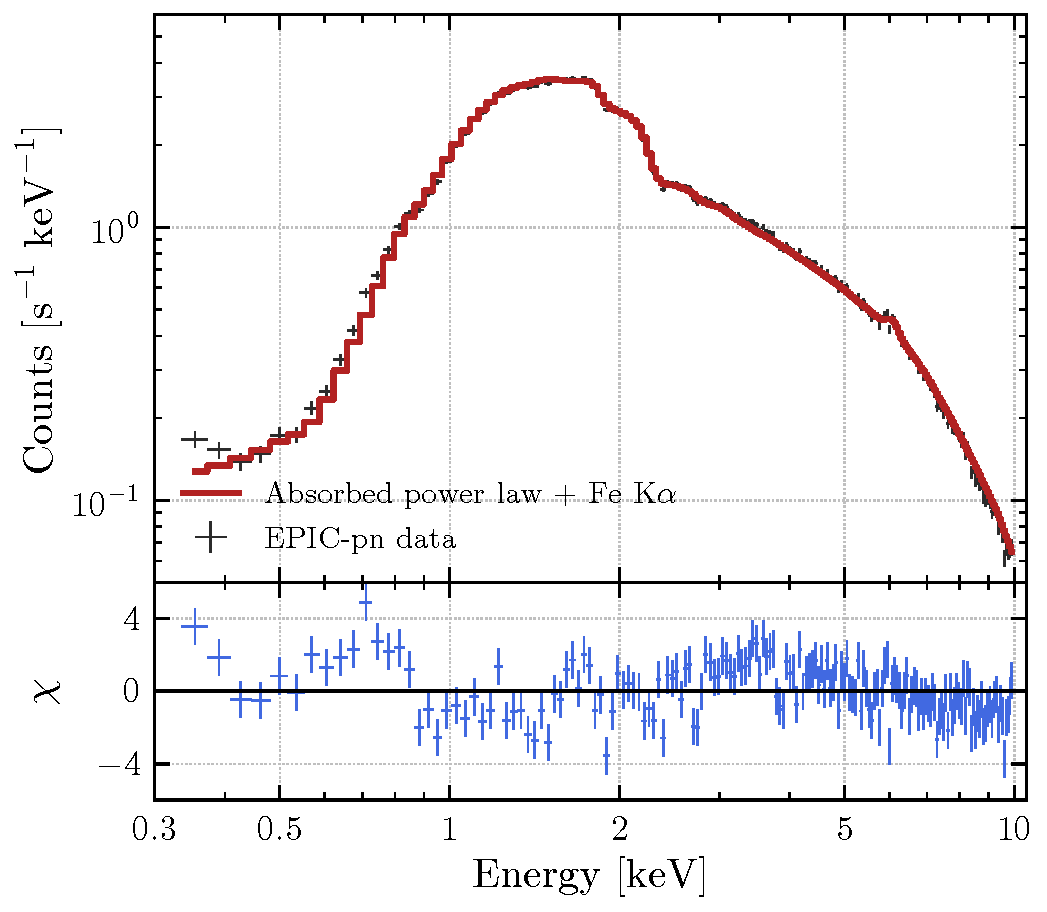
\includegraphics[width=0.72\textwidth]{figures/fig04_fit_powerlaw_FeKa.pdf}
\caption{EPIC-pn spectrum fitted with an absorbed power law plus a Gaussian Fe\,K$\alpha$ emission line (\texttt{tbabs$\times$(zpowerlw+zgauss)}). Lower panel: residuals in units of $\sigma$.}
\label{fig:fitfe}
\end{figure}

\begin{figure}[!htbp]
\centering
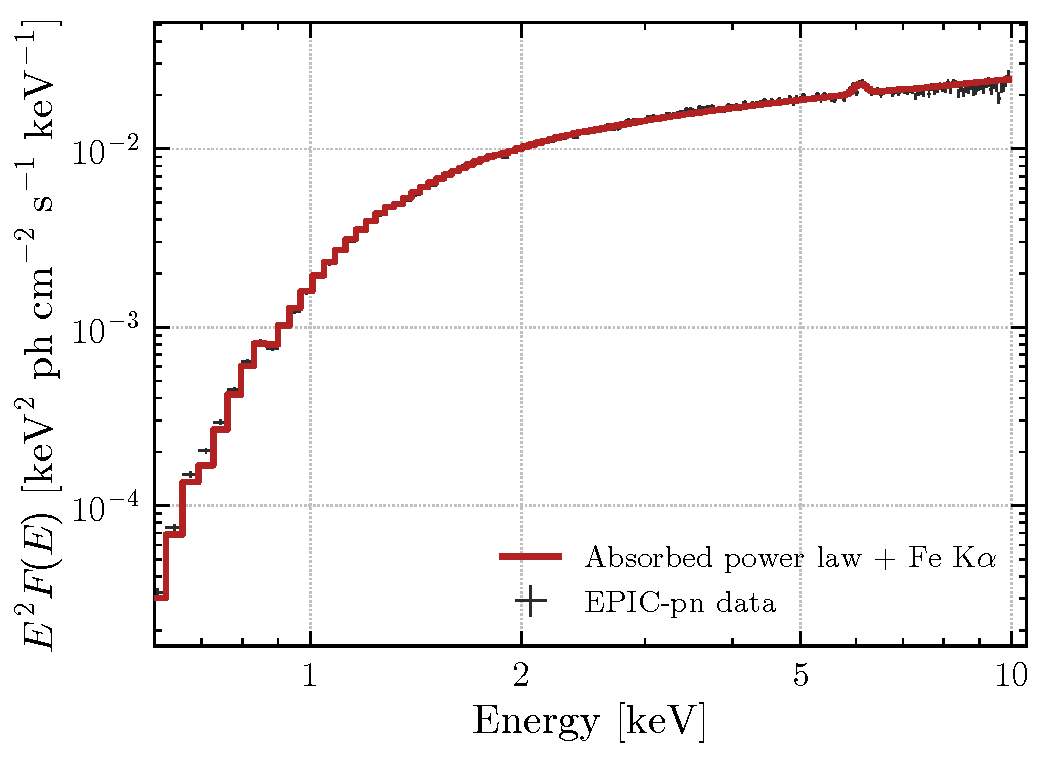
\includegraphics[width=0.72\textwidth]{figures/fig05_unfolded_spectrum.pdf}
\caption{Unfolded $E^2F(E)$ spectrum and best-fitting absorbed power law plus Fe\,K$\alpha$ model, shown above 0.6\,keV. The rising $E^2F(E)$ reflects $\Gamma<2$; the curvature below 2\,keV is due to absorption.}
\label{fig:unf}
\end{figure}

\subsection{Fluxes, luminosity and flux density}

Observed fluxes were computed from the best-fitting model with 90 per cent errors from 1000 simulations of the fit covariance matrix (\texttt{flux ... err 1000 90}). Unabsorbed fluxes and rest-frame luminosities, with errors, were obtained by refitting with the convolution models \texttt{cflux} and \texttt{clumin} applied to the unabsorbed emission, \texttt{tbabs$\times$cflux(zpowerlw+zgauss)} and \texttt{tbabs$\times$clumin(zpowerlw+zgauss)}, so that $\log F$ and $\log L$ become fit parameters. As a cross-check, the luminosity was also computed independently as $L=4\pi D_L^2 F_{\rm unabs}(1+z)^{\Gamma-2}$; the two agree to better than 0.5 per cent ($2.70$ versus $2.72\times10^{44}$\,erg\,s$^{-1}$ in 2--10\,keV). The monochromatic flux density at 1\,keV ($2.42\times10^{17}$\,Hz) was obtained from the model flux in 0.99--1.01\,keV.

\subsection{Best-fit parameters}

Table~\ref{tab:fit} summarises all spectral parameters for both models.

\begin{table}[H]
\centering
\caption{Best-fitting EPIC-pn spectral parameters of 3C\,111 (0.3--10\,keV, $z=0.049$, 177 spectral bins). Errors are 90 per cent confidence ($\Delta\chi^2=2.706$). Luminosities are in the rest frame and corrected for absorption; the line energy is in the rest frame.}
\label{tab:fit}
\small
\begin{tabular}{llcc}
\toprule
Quantity & Unit & Absorbed power law & Absorbed PL + Fe K$\alpha$ \\
\midrule
\multicolumn{4}{l}{\textit{Absorption and continuum}}\\
$\nh$ & $10^{22}$ cm$^{-2}$ & $1.054^{+0.009}_{-0.009}$ & $1.058^{+0.009}_{-0.009}$ \\
$\Gamma$ & -- & $1.627^{+0.008}_{-0.008}$ & $1.635^{+0.008}_{-0.008}$ \\
Normalisation (1 keV) & $10^{-2}$ ph keV$^{-1}$ cm$^{-2}$ s$^{-1}$ & $1.150^{+0.012}_{-0.012}$ & $1.158^{+0.013}_{-0.013}$ \\[3pt]
\multicolumn{4}{l}{\textit{Fe K$\alpha$ emission line}}\\
Energy (rest) & keV & -- & $6.378^{+0.050}_{-0.051}$ \\
Width $\sigma$ & keV & -- & $0.124^{+0.055}_{-0.055}$ \\
Normalisation & $10^{-5}$ ph cm$^{-2}$ s$^{-1}$ & -- & $2.39^{+0.70}_{-0.65}$ \\
Equivalent width & eV & -- & $41^{+12}_{-12}$ \\[3pt]
\multicolumn{4}{l}{\textit{Fit statistic}}\\
$\chi^2$/dof & -- & $433.9/174$ & $388.3/171$ \\
$\chi^2_\nu$ & -- & $2.49$ & $2.27$ \\[3pt]
\multicolumn{4}{l}{\textit{Observed (absorbed) flux}}\\
$F$ (0.3--10 keV) & $10^{-11}$ \cgs & $5.286^{+0.021}_{-0.021}$ & $5.282^{+0.021}_{-0.022}$ \\
$F$ (2--10 keV) & $10^{-11}$ \cgs & $4.594^{+0.020}_{-0.021}$ & $4.590^{+0.020}_{-0.021}$ \\
$F$ (0.5--2 keV) & $10^{-11}$ \cgs & $0.691^{+0.003}_{-0.003}$ & $0.692^{+0.003}_{-0.003}$ \\[3pt]
\multicolumn{4}{l}{\textit{Unabsorbed flux}}\\
$F$ (0.3--10 keV) & $10^{-11}$ \cgs & $7.868$ & $7.888^{+0.037}_{-0.036}$ \\
$F$ (2--10 keV) & $10^{-11}$ \cgs & $4.867$ & $4.863^{+0.021}_{-0.021}$ \\[3pt]
\multicolumn{4}{l}{\textit{Luminosity (rest frame, unabsorbed)}}\\
$L$ (2--10 keV) & $10^{44}$ erg s$^{-1}$ & $2.72$ & $2.70^{+0.01}_{-0.01}$ \\
$L$ (0.3--10 keV) & $10^{44}$ erg s$^{-1}$ & $4.39$ & $4.39^{+0.02}_{-0.02}$ \\[3pt]
\multicolumn{4}{l}{\textit{Flux density at 1 keV}}\\
$F_\nu$ (observed) & $\mu$Jy & $1.13$ & $1.13$ \\
$F_\nu$ (unabsorbed) & $\mu$Jy & $7.05$ & $7.10$ \\
\bottomrule
\end{tabular}
\end{table}

\subsection{Fit quality}
\label{sec:quality}

Even for the best-fitting model the reduced $\chi^2$ is 2.27, formally a poor fit. With $3.5\times10^5$ counts the statistical errors per bin are only 1--3 per cent, so residual calibration uncertainties of a few per cent are enough to raise $\chi^2$ substantially. To locate the excess, the best-fitting model was refitted in restricted energy bands (Table~\ref{tab:diag}). Above 3\,keV, where absorption has no effect and $\nh$ was therefore frozen, the model is statistically acceptable ($\chi^2_\nu=1.02$, null-hypothesis probability 0.41) and the line energy is unchanged (6.38\,keV). The excess $\chi^2$ is thus confined to 0.3--3\,keV.

\begin{table}[H]
\centering
\caption{Fits of the absorbed power law + Fe\,K$\alpha$ model in different energy bands.}
\label{tab:diag}
\begin{tabular}{lcccc}
\toprule
Band (keV) & $\chi^2$/dof & $\chi^2_\nu$ & $\nh$ ($10^{22}$ cm$^{-2}$) & $\Gamma$ \\
\midrule
0.3--10 & 388.3/171 & 2.27 & 1.058 & 1.635 \\
0.5--10 & 370.7/166 & 2.23 & 1.059 & 1.635 \\
3--10 & 108.6/106 & 1.02 & 1.059 (frozen) & 1.724 \\
\bottomrule
\end{tabular}
\end{table}

The soft-band residuals (Fig.~\ref{fig:fitfe}) are systematically positive at 0.57--0.85\,keV and negative at 0.88--1.5\,keV, with an additional dip near the Si K edge at 1.84\,keV. A structured pattern of this kind is produced by a small shift of the energy scale rather than by a missing physical component. \cite{ballo11} found, for this same observation, that the pn data are affected by \emph{X-ray loading}: at high count rates source photons enter the on-board offset map, shifting event energies to lower values and moving events from double to single patterns. The pattern fractions of Fig.~\ref{fig:epat} show a mild deficit of doubles and excess of singles relative to the expectation, consistent with this effect, for which no reliable correction exists. \cite{ballo11} therefore excluded pn data below 1\,keV. In the present analysis the full band is retained to constrain $\nh$, and the hard-band parameters are regarded as the more robust.

A consequence is that the photon index depends on the band used: $\Gamma=1.635$ in 0.3--10\,keV and $1.72$ in 3--10\,keV. This systematic difference is ten times larger than the statistical error and should be considered the realistic uncertainty on $\Gamma$. The fluxes and luminosity are much less sensitive: they change by less than 1 per cent between models.

\section{Comparison with Previous Work}

\cite{ballo11} analysed the same observation, combining pn (1--10\,keV, single events only) and MOS2 (0.4--10\,keV) data, with a cut-off power law plus a weak reflection component and Fe\,K$\alpha$ and K$\beta$ lines. Table~\ref{tab:comp} compares their results with this work.

\begin{table}[H]
\centering
\caption{Comparison with \citet{ballo11} for ObsID 0552180101.}
\label{tab:comp}
\small
\begin{tabular}{lcc}
\toprule
Quantity & This work & \citet{ballo11} \\
\midrule
$\nh$ ($10^{22}$ cm$^{-2}$) & $1.058\pm0.009$ & $1.04\pm0.01$ \\
$\Gamma$ & 1.635 (0.3--10 keV), 1.72 (3--10 keV) & $1.58\pm0.01$ \\
Fe K$\alpha$ energy (keV, rest) & $6.38\pm0.05$ & $6.41\pm0.03$ \\
Fe K$\alpha$ $\sigma$ (eV) & $124\pm55$ & $89^{+53}_{-51}$ \\
Fe K$\alpha$ flux ($10^{-5}$ ph\,cm$^{-2}$\,s$^{-1}$) & $2.39^{+0.70}_{-0.65}$ & $2.34^{+0.59}_{-0.53}$ \\
Fe K$\alpha$ EW (eV) & $41\pm12$ & $38^{+11}_{-9}$ \\
$F_{\rm obs}$ (0.5--2 keV; $10^{-12}$ cgs) & 6.92 & $6.83^{+0.07}_{-0.11}$ \\
$F_{\rm obs}$ (2--10 keV; $10^{-11}$ cgs) & 4.59 & $4.83^{+0.11}_{-0.09}$ \\
$L$ (2--10 keV, $10^{44}$ erg s$^{-1}$) & 2.70 & $2.75^{+0.06}_{-0.05}$ \\
\bottomrule
\end{tabular}
\end{table}

The column density, the line parameters and the soft-band flux agree within the errors. The 2--10\,keV flux of this work is about 5 per cent lower, which is within typical cross-calibration differences between EPIC cameras and between event-pattern selections. The photon index depends on the continuum model, the cameras and the energy band. \cite{ballo11} used a power law with an exponential cut-off at 100\,keV, which curves the spectrum downwards and therefore requires a flatter intrinsic index to reproduce the same observed slope; their simpler joint fit to the same XMM-Newton data gives $\Gamma=1.61\pm0.01$, close to the full-band value found here. The luminosities agree to 2 per cent despite their slightly different cosmology ($H_0=71$).

\section{Summary and Discussion}

\begin{table}[H]
\centering
\caption{Summary of Part C results (best-fitting model).}
\label{tab:summary}
\begin{tabular}{ll}
\toprule
Spectral products & \texttt{pn\_src\_grp.pi}, \texttt{pn\_bkg\_spec.pi}, \texttt{pn\_src.rmf}, \texttt{pn\_src.arf} \\
Net count rate & $8.192\pm0.014$ counts s$^{-1}$ (livetime 42.2 ks) \\
Background fraction & $<1$ per cent \\
Pile-up & none (Part A: $s=1.003\pm0.004$, $d=0.991\pm0.005$) \\
Best-fitting model & \texttt{tbabs$\times$(zpowerlw+zgauss)}, 0.3--10 keV \\
$\nh$ & $(1.058\pm0.009)\times10^{22}$ cm$^{-2}$ \\
$\Gamma$ & $1.635\pm0.008$ (stat.), 1.63--1.72 (band-dependent) \\
Fe K$\alpha$ & $E=6.38\pm0.05$ keV, EW $=41\pm12$ eV \\
$F_{\rm obs}$ / $F_{\rm unabs}$ (2--10 keV) & $4.59$ / $4.86\times10^{-11}$ \cgs \\
$L$ (2--10 keV) & $(2.70\pm0.01)\times10^{44}$ erg s$^{-1}$ \\
$F_\nu$ (1 keV) & 1.13 $\mu$Jy observed, 7.10 $\mu$Jy unabsorbed \\
Fit statistic & $\chi^2/\mathrm{dof}=388.3/171$; 3--10 keV: $108.6/106$ \\
\bottomrule
\end{tabular}
\end{table}

The EPIC-pn spectrum of 3C\,111 is well described by a heavily absorbed, hard power law with a weak, moderately broad Fe\,K$\alpha$ line. The main results relevant for the physical interpretation (Part~D) are:

\begin{itemize}
\item \textbf{Absorption.} The column $\nh\approx1.06\times10^{22}$\,cm$^{-2}$ is about 3.6 times the Galactic H\,\textsc{i} column towards 3C\,111 ($2.9\times10^{21}$\,cm$^{-2}$; \citealt{kalberla05}). The line of sight crosses a Galactic molecular cloud, and the total Galactic column, including molecular gas, can reach $\sim1.3\times10^{22}$\,cm$^{-2}$ \citep{ballo11,tombesi17}. The measured absorption is therefore consistent with being mostly Galactic.
\item \textbf{Continuum.} $\Gamma\approx1.6$--1.7 is flatter than the $\Gamma\approx1.9$ typical of radio-quiet Seyfert galaxies, in agreement with previous X-ray studies of this source.
\item \textbf{Fe K$\alpha$ line.} The line is required at high significance but is weak (EW $\approx40$\,eV), as found for other broad-line radio galaxies.
\item \textbf{Luminosity.} $L_{2-10}\approx2.7\times10^{44}$\,erg\,s$^{-1}$ places 3C\,111 among luminous, radiatively efficient AGN.
\end{itemize}

\paragraph{Caveats and choices.}
\begin{itemize}
\item A single absorber was used for Galactic and intrinsic absorption. With the Galactic column uncertain by several $10^{21}$\,cm$^{-2}$, the pn data cannot separate the two.
\item The soft band is affected by instrumental systematics (Section~\ref{sec:quality}); the reduced $\chi^2$ of the full-band fit reflects these rather than a missing physical component, as shown by the acceptable 3--10\,keV fit. No systematic error was added to the data.
\item The Fe\,K$\beta$ line (7.06\,keV) was not modelled separately; part of the fitted Gaussian width may be due to it.
\item No reflection continuum was included, as it cannot be constrained without data above 10\,keV.
\item Only EPIC-pn data were used. The MOS cameras could provide an independent check of the soft-band calibration.
\end{itemize}

\paragraph{Products.} \texttt{pn\_src\_spec.pi}, \texttt{pn\_bkg\_spec.pi}, \texttt{pn\_src\_grp.pi}, \texttt{pn\_src.rmf}, \texttt{pn\_src.arf}, the best-fit model files \texttt{best\_fit\_m1.xcm} and \texttt{best\_fit\_m2.xcm}, the parameter file \texttt{fit\_results.txt}, and all figures and scripts, in \texttt{\textasciitilde/sas/SPASE/part\_c}.

\begin{thebibliography}{9}
\bibitem[Ballo et al.(2011)]{ballo11} Ballo, L., Braito, V., Reeves, J.~N., Sambruna, R.~M., \& Tombesi, F. 2011, MNRAS, 418, 2367 -- The high-energy view of the broad-line radio galaxy 3C\,111.
\bibitem[Kalberla et al.(2005)]{kalberla05} Kalberla, P.~M.~W., et al. 2005, A\&A, 440, 775 -- The Leiden/Argentine/Bonn (LAB) survey of Galactic H\,\textsc{i}.
\bibitem[Protassov et al.(2002)]{protassov02} Protassov, R., van Dyk, D.~A., Connors, A., Kashyap, V.~L., \& Siemiginowska, A. 2002, ApJ, 571, 545 -- Statistics, handle with care.
\bibitem[Tombesi et al.(2017)]{tombesi17} Tombesi, F., et al. 2017, ApJ, 842, 64 -- Excess Galactic molecular absorption toward the radio galaxy 3C\,111.
\bibitem[Verner et al.(1996)]{verner96} Verner, D.~A., Ferland, G.~J., Korista, K.~T., \& Yakovlev, D.~G. 1996, ApJ, 465, 487 -- Atomic data for astrophysics: photoionization cross sections.
\bibitem[Wilms et al.(2000)]{wilms00} Wilms, J., Allen, A., \& McCray, R. 2000, ApJ, 542, 914 -- On the absorption of X-rays in the interstellar medium.
\bibitem[Arnaud(1996)]{arnaud96} Arnaud, K.~A. 1996, ASP Conf. Ser. 101, 17 -- XSPEC: the first ten years.
\bibitem[Gabriel et al.(2004)]{gabriel04} Gabriel, C., et al. 2004, ASP Conf. Ser. 314, 759 -- The XMM-Newton SAS.
\end{thebibliography}

\clearpage
\appendix

\section{Complete Analysis Command Log}

\begin{lstlisting}[language=bash]
# ---- environment (SAS initialised with sasenv) ----
cd ~/sas/SPASE/part_c
export SAS_CCFPATH=$HOME/sas/SPASE/CCF
export SAS_CCF=$HOME/sas/SPASE/ccf.cif
export SAS_ODF=$PWD/1683_0552180101_SCX00000SUM.SAS
mkdir -p scripts results figures/raw

# ---- missing calibration files (listed in ccf.cif, needed by rmfgen/arfgen) ----
grep -a -o "[A-Z0-9_]*_[0-9]\{4\}\.CCF" ../ccf.cif | sort -u > ../ccf_all_in_cif.txt
# download every EPN_*, XRT3_*, XMM_* file not yet present from
# https://heasarc.gsfc.nasa.gov/FTP/xmm/data/CCF/ into $SAS_CCFPATH

# ---- spectra, responses, grouping, pile-up check ----
./scripts/01_extract_spectrum.sh

# ---- check that the grouped spectrum points to its auxiliary files ----
fkeyprint pn_src_grp.pi+1 BACKFILE      # pn_bkg_spec.pi
fkeyprint pn_src_grp.pi+1 RESPFILE      # pn_src.rmf
fkeyprint pn_src_grp.pi+1 ANCRFILE      # pn_src.arf

# ---- fit, figures, table (03_make_plots.py also redraws the epatplot fractions) ----
pip install beautifultable astropy numpy matplotlib pymupdf
./scripts/run_partC.sh 2>&1 | tee results/run_partC_terminal.txt

# ---- band-dependent fit diagnostics ----
xspec <<< "@scripts/05_diagnostics.xcm" > /dev/null 2>&1
cat results/diagnostics.txt
\end{lstlisting}

\section{Scripts}
\label{app:scripts}

\subsection{01\_extract\_spectrum.sh}
\lstinputlisting[language=bash]{../scripts/01_extract_spectrum.sh}

\subsection{02\_fit\_spectrum.xcm}
\lstinputlisting[language=tcl]{../scripts/02_fit_spectrum.xcm}

\subsection{05\_diagnostics.xcm}
\lstinputlisting[language=tcl]{../scripts/05_diagnostics.xcm}

\subsection{run\_partC.sh}
\lstinputlisting[language=bash]{../scripts/run_partC.sh}

\subsection{03\_make\_plots.py}
\lstinputlisting[language=Python]{../scripts/03_make_plots.py}

\subsection{04\_results\_table.py}
\lstinputlisting[language=Python]{../scripts/04_results_table.py}

\end{document}
